\documentclass{assignment-373}
\usepackage{mathabx}
\usepackage{tikz}
\usepackage{graphicx}


\anum{8}
\course{CSC373}
\duedate{WEDNESDAY, Dec 2, 2020}
\filename{ps8.pdf, ps8.tex}

\begin{document}

\think


\textbf{[15 points]}

A wireless network company has a number of sensors $s_1, \dots, s_n$, each located at coordinates $(x_i, y_i) \in \mathbb{R}^2$ on some map. The company would like to make the sensors more reliable by assigning each sensor $s_i$ a backup set $B_i \subseteq \{s_1, \dots, s_n\} - \{s_i\}$ so that if $s_i$ fails, a sensor in $B_i$ can be used instead. The company decides that:

\begin{itemize}
    \item Each backup set $B_i$ must contain sensors within distance at most $d$ from $s_i.$
    \item Each backup set $B_i$ must contain at least $r$ backup sensors.
    \item Every sensor $s_i$ must belong at most $b$ backup sets. 
\end{itemize}

\begin{enumerate}
\item \textbf{(7 points)} Given the sensors, their coordinates, and the parameters $d, r, b$ described, design an algorithm to output the backup sets for each sensor, or reports that choosing backup sets is not possible with the given parameters.\\\\
    Our algorithm consists of the following steps:\\\\
    Step 1:\\
    \phantom{=} \phantom{=} First we calculate the distance between each sensor. If the distance between two sensors is less than or equal to d, then one of the sensors can be the other sensor's backup sensor, and vice versa. So we create a dictionary to store these sensors, where the key are the name of the sensors, and the value would be a list containing the candidates for the backup sensors for that sensor.\\\\
    \\
    \\
    \\
    \\
    \\
    \\
    \\
    Step 2:\\
    \phantom{=} \phantom{=} We create a directed graph G with a single source point s, connect s to each sensors with a forward edge with capacity b.\\
    \begin{center}
	    \textbf{Figure 1:}
	\end{center}
    \begin{center}
    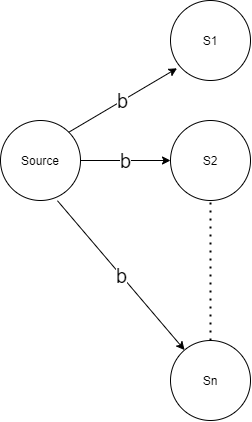
\includegraphics[width=5cm]{./g1.png}
    \end{center}
    Step 3:\\
	\phantom{=} \phantom{=} We create a list of backup sets. $B_{1}$ is the backup set of $S_{1}$, $B_{2}$ is the backup set of $S_{2}$.... Then build forward edges between each sensor and the corresponding backup sets (based on whether it can become the backup sensor of that backup set based on information from our dictionary) with capacity 1.
	\begin{center}
	    \textbf{Figure 2:}
	\end{center}
    \begin{center}
    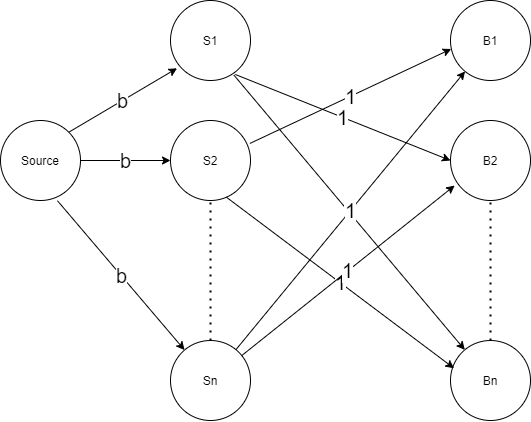
\includegraphics[width=10cm]{./g2.png}
    \end{center}
    
    \newpage
    Step 4:\\
    \phantom{=} \phantom{=} To finish the graph, we connect each element $B_i$ to the sink t with a capacity r in graph G. The final graph will look like that following:\\
    \begin{center}
    \textbf{Figure 3:}
    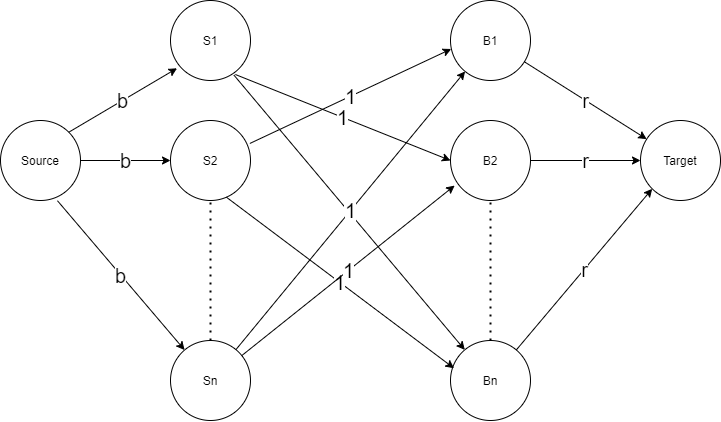
\includegraphics[width=15cm]{./G.png}
    \end{center}
	
	Step 5:\\
	\phantom{=} \phantom{=} Finally we run a ford-fulkerson algorithm to find out the maximum flow of the graph. If the maximum flow is less then $len(sensors) * r$, this means that some backup set $B_{i}$ does not have enough backup sensors (less than r backup sensors). So we will not able to find proper backup sets. Otherwise we return B, which means we find the backup sets successfully.\\\\
	
	\textbf{pseudo-code:}  
    \begin{python}
def distance(coord1, coord2):
	"""
	calculate the distance between two coordinates
	"""
 	return sqrt((abs(coord1[0] - coord2[0]) ** 2) + 
 	(abs(coord1[1] - coord2[1]) ** 2))


def Bottleneck (p,f):
    return min (cf(u,v))


def AUGMENT (f,p,sensors,B):
    let b <- Bottleneck (p,f)
    for all (u,v) in p:
        if (u,v) is a forward edge :
            f(e) <- f(e) + b
            if u in sensors and v in B:
                add sensor "u" to backup set "v"
        if (u,v) is a backward edge :
            f(e) <- f(e) - b
            if u in sensors and v in B:
                remove sensor "u" from backup set "v"
    return f


def Max_Flow (G,s,t,sensors,B):
    set f(e)<- 0 for all e in E(G)
    while there exist s-t path in Gf:
        p = a simple (s,t) path in Gf
        f' <- AUGMENT (f,p, sensors,B)
        set f <- f'
        compute Gf '
        set Gf <- Gf '
    return f


def backup_set(sensors, coordinates, d,r,b):
    # 1
    in_range = dict(key:sensors,  value:[])
    for i in range(sensors):
        for j in range(sensors):
            if j == i:
                continue
            if distance(coordinates[sensors[i]],
             coordinates[sensors[j]]) <= d:
                in_range[sensors[i]].append(sensors[j])
    
    # 2
    G  = (s,none) # a directed graph with only a source point s
    for i in sensors:
        build forward edge (s->i) with capacity(s->i)=b, and store in G
    
    # 3
    B = [B1,B2,B3....Bn] # A list of backup sets (use python list here)
    for i in sensors:
        for j in in_range[i]:
            build forward edge (j->B[i]) with capacity(j->B[i])=1, and store in G
     
    # 4
    for i in B:
        build forward edge (B[i]->t) with capacity(b[i]->t)=r, and store in G
    
    # 5 run Ford - Fulkerson
    MaxFlow = Max_Flow (G,s,t, sensors,B)
    if MaxFlow == len(sensors) * r:
        return B
    else:
        print("choosing backup sets is not 
        possible with the given parameters")
    return
    \end{python}

\item \textbf{(8 points)} Briefly justify the correctness and runtime of the algorithm designed in the previous part.

 \phantom{=} \phantom{=} To prove the correctness of our algorithm, let G be the flow graph we built using our algorithm from part (1), we will:\\
       \phantom{=} \phantom{=}  (1). Prove "if there exists backup set for each sensor, then max-flow(G) $= n*r$ where n is the total number of backup sets".\\
        \phantom{=} \phantom{=} (2). Prove "if max-flow(G) $= n*r$ where n is the total number of backup sets, then there exists backup set for each sensor".\\
         \phantom{=} \phantom{=} (3). Prove our python list of lists contains the correct backup sets with each list representing a backup set.\\
        
    (1). To prove this claim, let's assume that there exists a backup set for each sensor, then this implies that we have n backup sets with each backup set having at least r sensors.
    
    \phantom{=} \phantom{=} First, since r is the number of sensors that can be added to the backup set, and we cannot add part of the sensor to the set, nor produce part of the sensor and expect it to work. So, all flows are \textbf{integers}.
    
    \phantom{=} \phantom{=} Consider a max-flow in G,\\
    \phantom{=} \phantom{=} For each vertex $s_i$\\
    \phantom{=} \phantom{=} \phantom{=} (a). Capacity$(s,s_i)=b$, because each sensor can belong in \textbf{at most} b backup sets.\\
    \phantom{=} \phantom{=} \phantom{=} Then, flow$(s,s_i)\leq b$ or we go above our limit, which is not allowed.\\
    \phantom{=} \phantom{=} \phantom{=} Therefore, the conservation constraint holds for all $s_i$.\\
    \phantom{=} \phantom{=} \phantom{=} (b). Capacity$(s_i,B_j)=1$, because all sensors are unique and can only be added to \textbf{exactly} 1 time to a certain backup set, and flow$(s_i,B_j)=1$ \textbf{if and only if} the backup set for $s_j = B_j$ is within distance "d" of $s_i$ and $s_i$ hasn't being added to $B_j$ yet.\\
    \phantom{=} \phantom{=} \phantom{=} So, flow$(s,s_i)=\sum_{j=1}^{N}$flow$(s_i,B_j)$, as we will only add $s_i$ if another sensor is close enough and $s_i$ hasn't been added.\\
    \phantom{=} \phantom{=} \phantom{=} Then, there are as many $s_i$ been added as the number of sensors that are close to it, which implies flow\_in$(s_i)$=flow\_out$(s_i)$.\\
    \phantom{=} \phantom{=} \phantom{=} Therefore, the conservation constraint holds.\\
    \\
    \phantom{=} \phantom{=} For each vertex $B_i$\\
    \phantom{=} \phantom{=} \phantom{=} (a). Capacity$(s_j,B_i)=1$, and flow$(s_j,B_i)=1$ \textbf{if and only if} $s_j$ is added to $B_i$ and flow$(s,s_j)\leq$capacity$(s,s_j)$ (in other words, the mandatory upper limit "b" for $s_j$ hasn't been reached yet).\\
    \phantom{=} \phantom{=} \phantom{=} So, flow$(s_j,B_i)\epsilon\{0,1\}$(0 when $s_i$ is not assigned $B_j$, or 1 otherwise), and since capacity$(s_j,B_i)=1$, flow$(s_j,B_i)\leq$capacity$(s_j,B_i)$.\\
    \phantom{=} \phantom{=} \phantom{=} Therefore, the capacity constraint holds.\\
    \phantom{=} \phantom{=} \phantom{=} (b). Capacity$(B_i,t)=r$ and flow$(B_i,t)=r$ \textbf{if and only if} r "qualified" sensors are added to backup set $B_i$.\\
    \phantom{=} \phantom{=} \phantom{=} And flow$(B_i,t)=\sum_{j=1}^{N}$flow$(s_j,B_i)$ for some $s_j$ depending on the backup set $S_i$, so flow\_in$(c_i)=$flow\_out$(c_i)$.\\
    \phantom{=} \phantom{=} \phantom{=} Therefore, we conclude that the conservation constraint holds.\\
    \\
    Now, by proving the 2 constraints hold on all internal vertices, we have shown that the Ford-Fulkerson algorithm will terminate and returns the maximum flow to us.\\
    
    \phantom{=} \phantom{=} Then, by construction of G, we know that max-flow(G) = "the total number of sensors that belong in a backup set" = m for some integer m. Out of the n backup sets in total, we need at least r sensors in every set to make the statement true, so we need at least $n*r$ sensors that are added to our backup sets to make the claim hold.\\
    \phantom{=} \phantom{=} Moreover, due to the capacity$(B_i,t)=r$, we upper-bound our backup set's cardinality by r, so we only need to check if the maxflow(G) = m to know if we have a working group of backup sets.\\
    \phantom{=} \phantom{=} Hence, if $m = n*r$, then we satisfies the conditions and proves that there exists a backup set for each sensor.\\
    \\
    (2). Similar to the part (2), we prove that the maxflow(G) = "the total number of sensors that belong in a backup set" = m. Then if $m = n*r$ where n="number of sensor" and r="mandatory limit for a single sensor to exist in multiple backup sets", then by construction of G, we know that there are at least $n*r$ sensors that belong in a backup set, and precisely each backup set contain \textbf{exactly} r "qualified" sensors, which finishes our proof for this claim. (We can add more "qualified" sensor to a backup set, but we will threshold it to r)\\
    
    (3). As we progress through the algorithm, our Augment function will add each candidate sensor $s_i$ to the corresponding backup set.\\
    \phantom{=} \phantom{=} If we used a backward edge to "undo" a previous choice, then our Augment function will also take out the sensor based on the "undo" path. (Which is also the reason why a greedy approach will likely to fail at this problem).\\
    \phantom{=} \phantom{=} So, by the end of the algorithm when we have explored all possible path, we will have the correct sensors in the correct backup sets.\\
    
    Therefore, by proving all 3 claims, we have shown that the algorithm is correct.\\
    
    \textbf{Time complexity:}\\
    \phantom{=} \phantom{=} We first consider the runtime of building the flow-graph G:\\
    \phantom{=} \phantom{=}\phantom{=} (1). initializing all vertices in G and connect each $s_i$ to s and each $B_j$ to t. (O(1+n+n+1)$=>$O(n) where n="number of sensors")\\
    \phantom{=} \phantom{=}\phantom{=} (2). build edges based on each sensor's distance. ($O(n(n-1))=>O(n^2)$, worst case being r=n-1, and all n sensors are within distance of one another).\\
    \phantom{=} \phantom{=} So, the total time complexity of building a graph is "O(n)+$O(n^2)=>O(n^2)$".\\
    \\
    \phantom{=} \phantom{=}Our modification to the BFS algorithm(checking if $(B_i, t)$ still has capacity for flow) takes constant time (look up in list and add to set), which is dominated by BFS's generic time complexity, which is then dominated by Ford-Fulkerson's complexity, so we will focus solely on complexity of Ford-Fulkerson.\\
    Time complexity of the FF algorithm depends on the max-flow on G and the number of edges in G. \\
    \phantom{=} \phantom{=}For the number of edges, let's consider the 4 layers of vertices in G.\\
    \phantom{=} \phantom{=}\phantom{=} $(s,s_i)$:   At this layer, we have n edges with n = "the total number of sensors". (check figure 1 in part (1) for details)\\
    \phantom{=} \phantom{=}\phantom{=} $(s_i,B_j)$: At this layer, we can have maximum number of $O(n^2)$ edges, which is the scenario where r=n-1 and all sensors are within distance of one another (then wee connect each $s_i$ with every backup set except $B_i$, check figure 2 in part (1) for details).\\
    \phantom{=} \phantom{=}\phantom{=} $(B_j,t)$: At this layer, we have n edges, where each edge represent the number of sensors added to that backup set.\\
    \\
    In total, $we have O(n + n^2 + n) = > O(n^2)$ edges. And the maximum max-flow is $r*n$, which is the case where all n backup sets meet the minimum requirement of sensors (the worst case scenario). In conclusion, we have $O(r*n*n^2) = O(rn^3)$ for our Ford-Fulkerson algorithm.\\
    
    Combining with the time complexity of building the flow-graph, we have $O(n^2)+O(rn^3)=>O(rn^3)$ time complexity, which satisfies the requirement.\\

\end{enumerate}

\end{document}



%%% Local Variables:
%%% mode: latex
%%% TeX-master: t
%%% End:
